% --------------------------------------------------------------
% This is all preamble stuff that you don't have to worry about.
% Head down to where it says "Start here"
% --------------------------------------------------------------

\documentclass[12pt]{article}

\usepackage[margin=1in]{geometry}
\usepackage{amsmath,amsthm,amssymb}
\usepackage{graphicx} %This allows to include eps figures
\usepackage{subcaption}
\usepackage[section]{placeins}
\usepackage{layout}
\usepackage{etoolbox}
\usepackage{mathabx}
\usepackage{animate}
\usepackage{array}
% This is to include code
\usepackage{listings}
\usepackage{xcolor}
\definecolor{dkgreen}{rgb}{0,0.6,0}
\definecolor{gray}{rgb}{0.5,0.5,0.5}
\definecolor{mauve}{rgb}{0.58,0,0.82}
\lstdefinestyle{Python}{
    language        = Python,
    basicstyle      = \ttfamily,
    keywordstyle    = \color{blue},
    keywordstyle    = [2] \color{teal}, % just to check that it works
    stringstyle     = \color{green},
    commentstyle    = \color{red}\ttfamily
}

\newenvironment{conditions}
  {\par\vspace{\abovedisplayskip}\noindent\begin{tabular}{>{$}l<{$} @{${}={}$} l}}
  {\end{tabular}\par\vspace{\belowdisplayskip}}

\newcommand{\N}{\mathbb{N}}
\newcommand{\Z}{\mathbb{Z}}

\newenvironment{theorem}[2][Theorem]{\begin{trivlist}
\item[\hskip \labelsep {\bfseries #1}\hskip \labelsep {\bfseries #2.}]}{\end{trivlist}}
\newenvironment{lemma}[2][Lemma]{\begin{trivlist}
\item[\hskip \labelsep {\bfseries #1}\hskip \labelsep {\bfseries #2.}]}{\end{trivlist}}
\newenvironment{exercise}[2][Exercise]{\begin{trivlist}
\item[\hskip \labelsep {\bfseries #1}\hskip \labelsep {\bfseries #2.}]}{\end{trivlist}}
\newenvironment{reflection}[2][Reflection]{\begin{trivlist}
\item[\hskip \labelsep {\bfseries #1}\hskip \labelsep {\bfseries #2.}]}{\end{trivlist}}
\newenvironment{proposition}[2][Proposition]{\begin{trivlist}
\item[\hskip \labelsep {\bfseries #1}\hskip \labelsep {\bfseries #2.}]}{\end{trivlist}}
\newenvironment{corollary}[2][Corollary]{\begin{trivlist}
\item[\hskip \labelsep {\bfseries #1}\hskip \labelsep {\bfseries #2.}]}{\end{trivlist}}



\begin{document}

% --------------------------------------------------------------
%                         Start here
% --------------------------------------------------------------

%\renewcommand{\qedsymbol}{\filledbox}

\title{Assignment 7}%replace X with the appropriate number
\author{Nalet Meinen and Pascal Wyss\\ %replace with your name
Finite Element Analysis I
}
\maketitle

\begin{figure}[!htb]
  \centering
  \vspace*{1cm}
  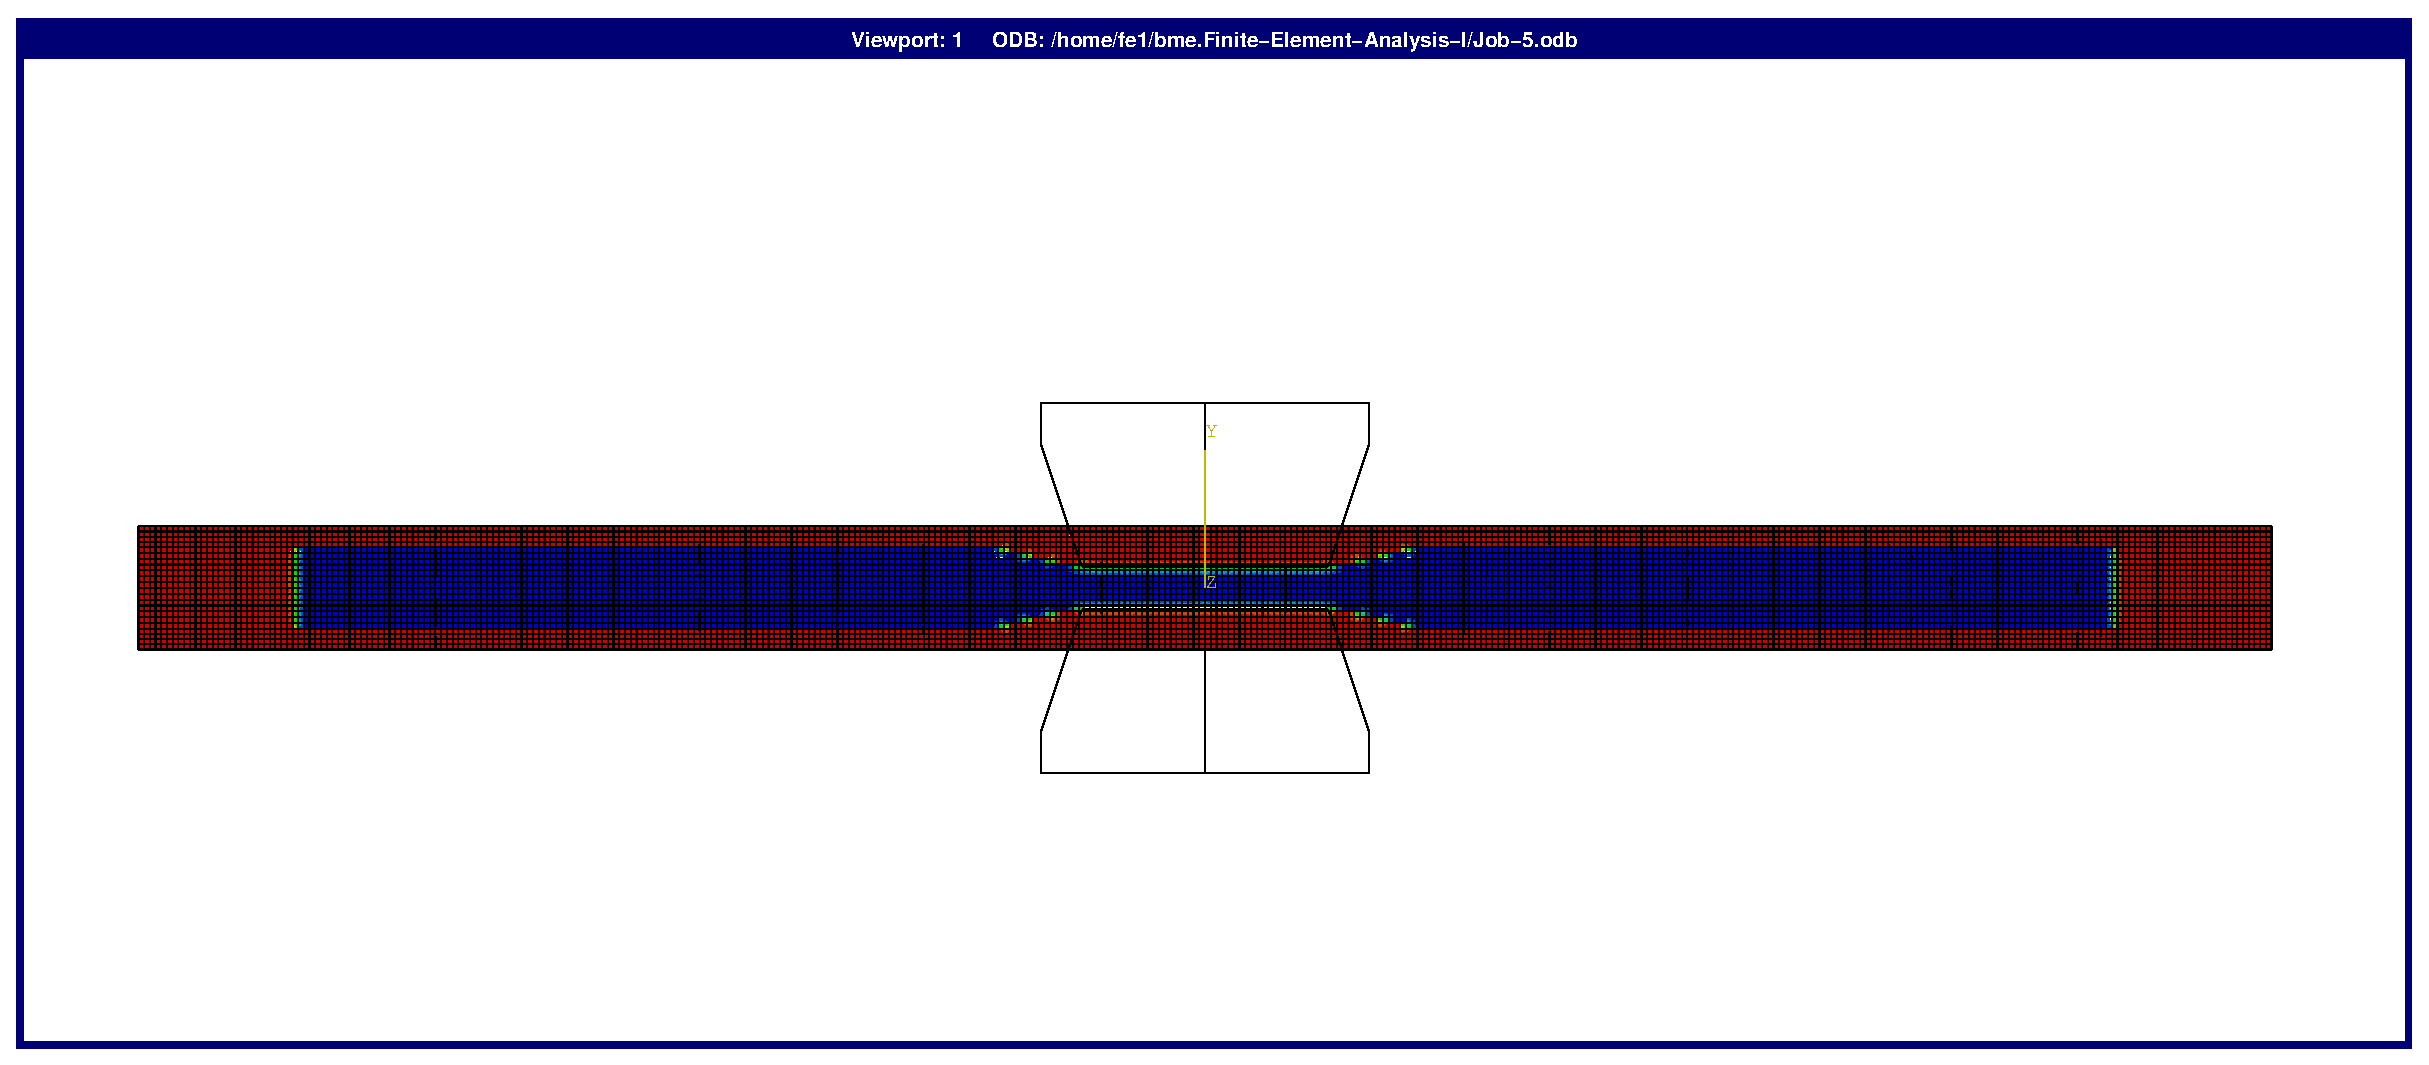
\includegraphics[trim={-3cm 2cm 2cm 2cm},clip,width=1.0\linewidth]{pics/titelbild}
  \label{fig:0}
\end{figure}

\newpage

\section*{Abstract}
In this assignment we investigate a cooling disc which is mounted on a shaft.
The occuring stresses after cooling are then assessed.

\tableofcontents
\pagebreak
\section{Introduction}

This assignment should show an introduction in thermo-mechanical simulations. With a numerical model of a disk and shaft,  the disc is heated up to increase its diameter, then cooled down to form an interference fit. This is a common procedure in mechanics to fit parts together (e.g. bearings on shafts). It is therefore interesting to know, by how much the disc has to be heated in order to get an inside diameter which fits over the shaft. In a practical application, this could be used to specify manufacturing tolerances.
Assuming the disc is uniform and isotropic (the same in different directions), the hole will expand in the same ratio as the metal. You can see this because of the thermal expansion equation.

\begin{equation}\label{eq:1}
  \delta l = l \cdot \alpha \cdot \delta t
\end{equation}
\begin{conditions}
  l         &  original length\\
  \delta l  &  thermal expansion\\
  \alpha    &  coefficient for heat expansion\\
  \delta t  &  temperature difference
\end{conditions}

\begin{figure}[!htb]
  \centering
  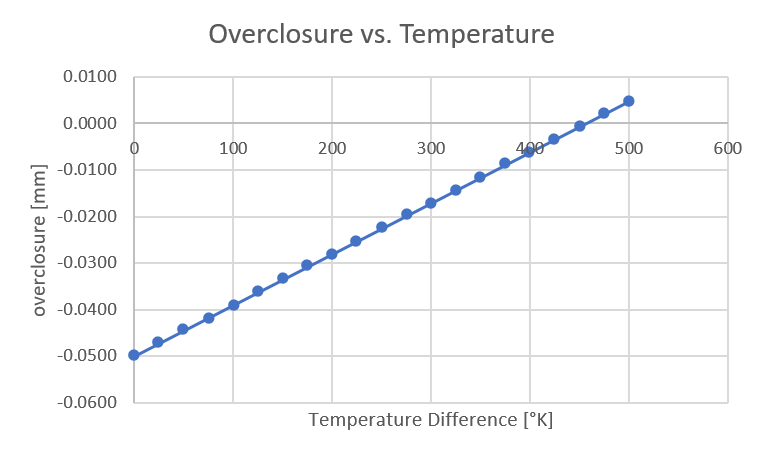
\includegraphics[width=0.9\linewidth]{pics/overclosure_temperature}
 \caption{overclosure}
  \label{fig:1}
\end{figure}



\newpage
\section{Methods}

\subsection{Diameter as Function of Temperature}

The inside diameter of the disc changes with temperature. The rate of change 
depends on the thermal heat expansion coefficient.




\subsection{Modelling}

\begin{figure}[!htb]
  \centering
  \begin{subfigure}{.5\textwidth}
    \centering
    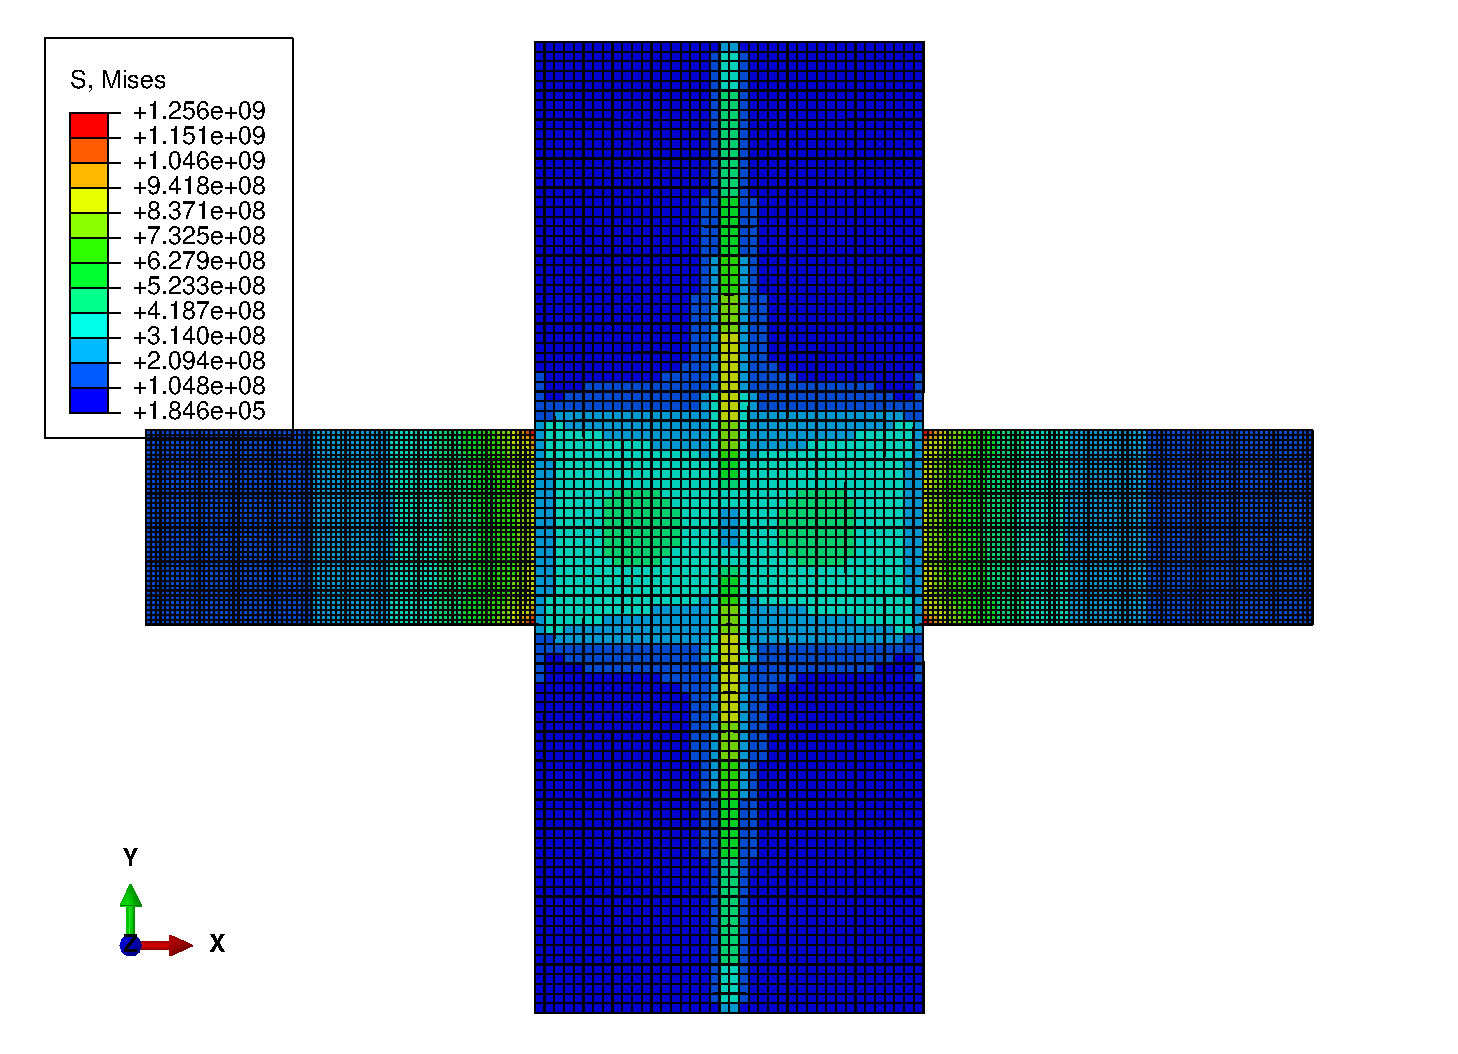
\includegraphics[width=0.95\linewidth]{pics/stress10}
    \caption{Overlap of 0.01 mm}
  \end{subfigure}%
  \begin{subfigure}{.5\textwidth}
    \centering
    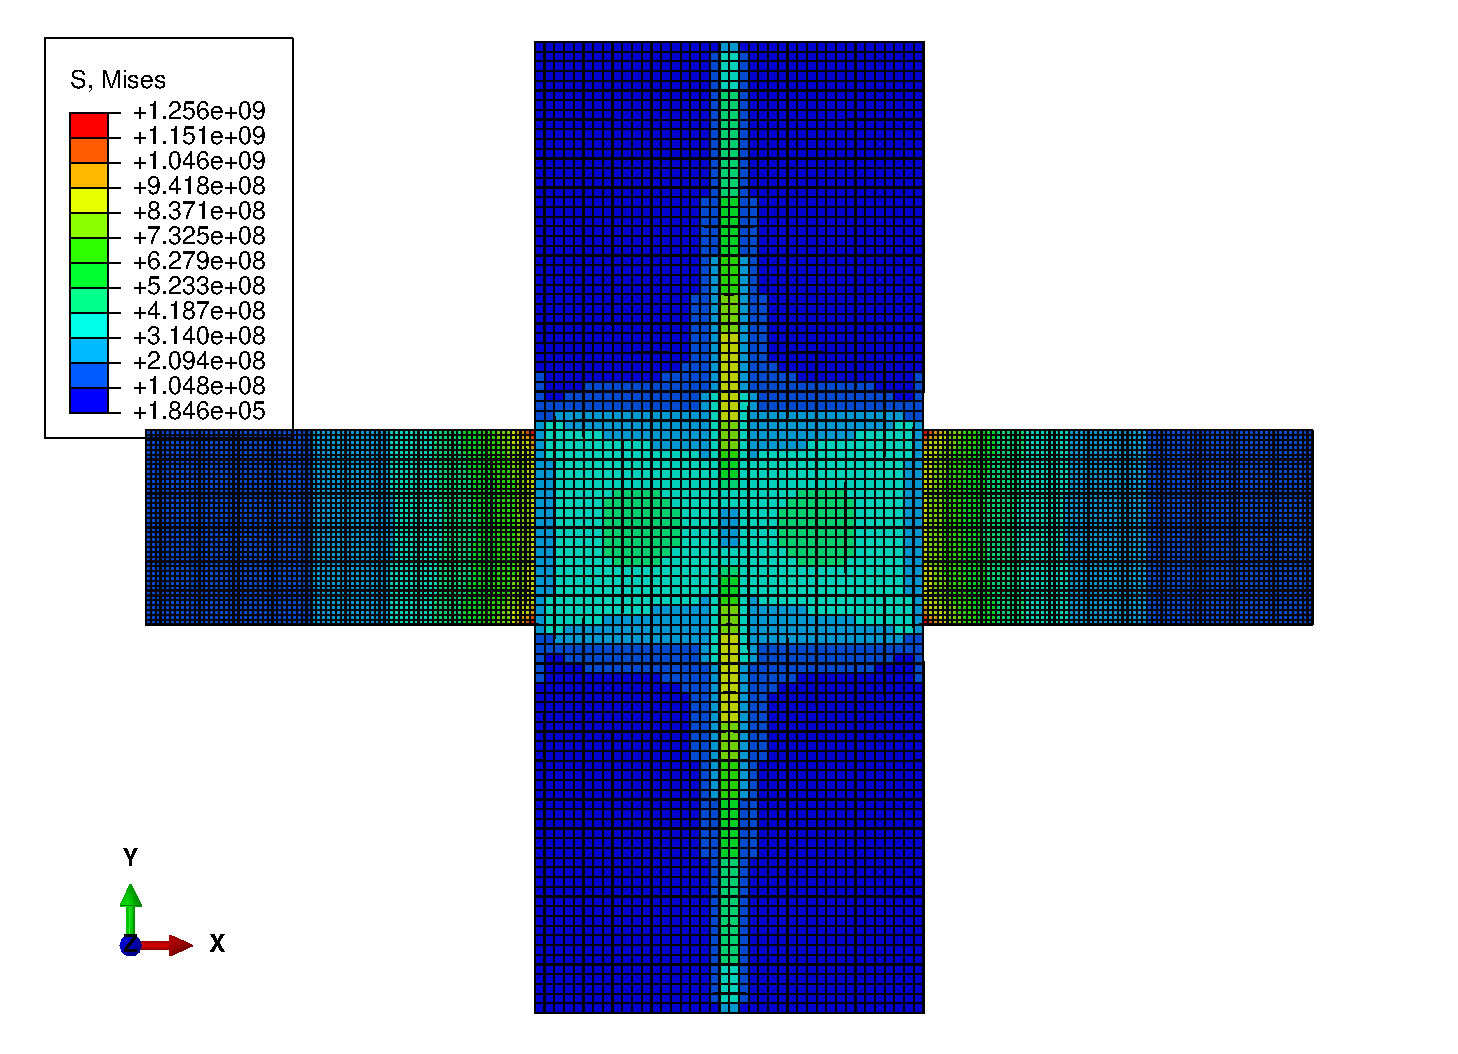
\includegraphics[width=0.95\linewidth]{pics/stress50}
    \caption{Overlap of 0.05 mm}
   \end{subfigure}
  \caption{Compason of overlap}
\end{figure}

It is important to sequence the model into different steps. 
Contacts are only activated after both
instances are clear of each other (after heating up the disc).



\begin{figure}[!htb]
  \centering
  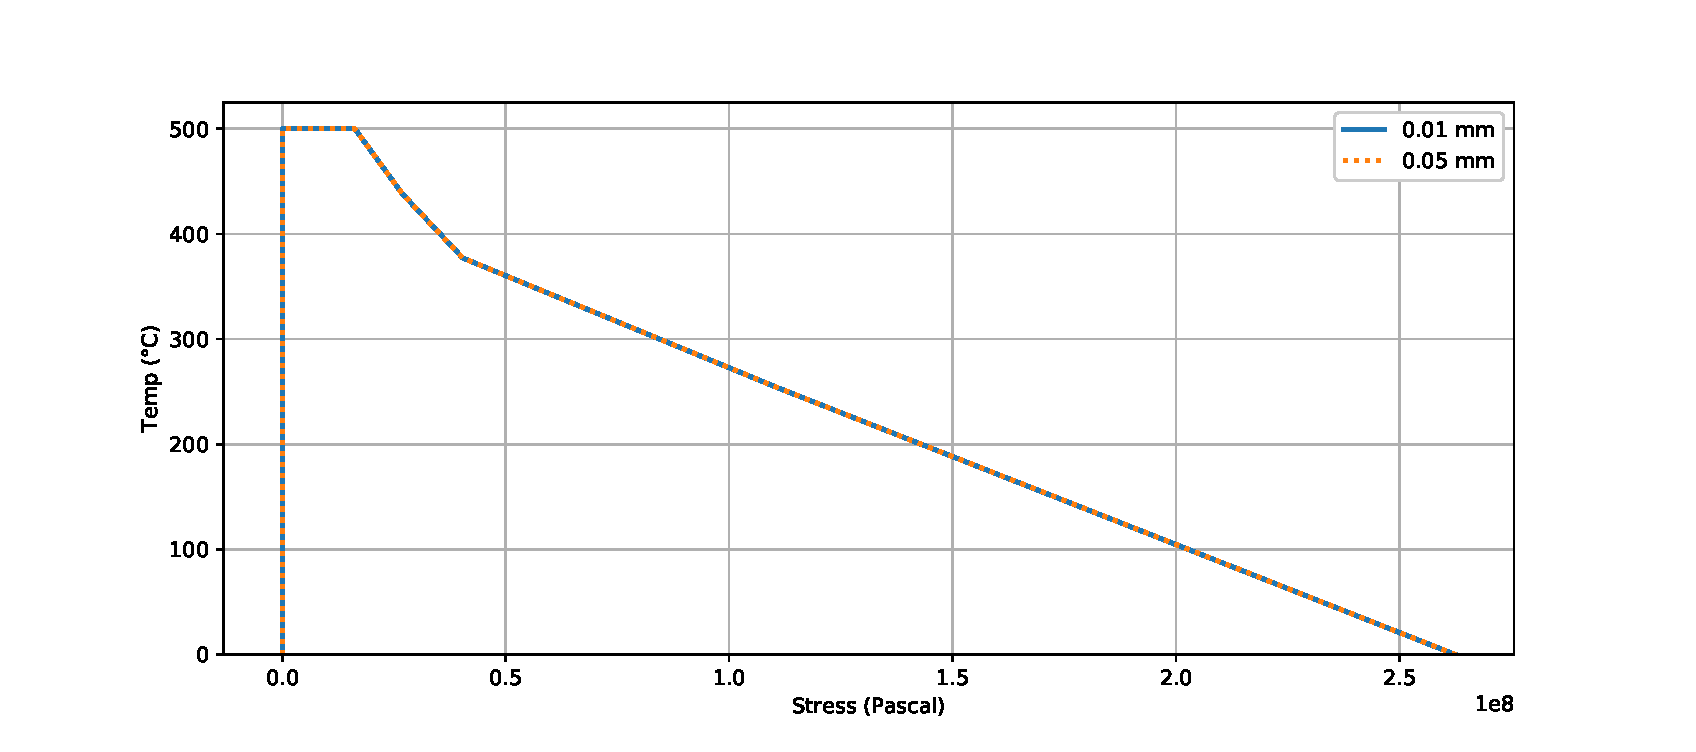
\includegraphics[width=0.9\linewidth]{pics/result10and50}
 \caption{overclosure}
  \label{fig:1}
\end{figure}




\pagebreak
\section{Results and Discussion}

The results vary greatly with different mesh sizes. Especially when using quilt plots,
results may differ quite heavily from one mesh to another, as there is no averaging between elements.
Quilt plots are good for evaluation on an element-by-element basis.
We reach a maximum mises sstress of around 1.2GPa, which is way below the plasic deformation threshold
for the shaft material, which lies at 200GPa. 
However, it is also possible that this maximum value of 1.2GPa comes from the thermal 
deformation of the part itself during heating up.
When thinkin about the real world application, it seems
reasonable that the maximum stresses stay in the elastic
region of the materials, because the shaft could not be reused after the diss (or bearing) would be removed.
The simulation with a smaller overlap of the parts shows no smaller stress value at the surface.
This is qulitatively a questionable result. We would assume, that by having a smaller
overclosure, lower stress values would result.
From a practical perspective, by dimensioning the overclosure to a certain
value (during manufacturing of the parts), engineers can influence the behaviour of the 
assembly, mainly its ability to withstand axial loads. 
We assume that there might be errors in the selection of the respective nodes for plotting,
or possibly in the material characteristics. However, due to lack of time we were not able to 
fully investigate further. Corrected results may follow in an appendix to this report.

\pagebreak
\begin{thebibliography}{9}
  \bibitem{Thin Circular Ring - Temperature and Expanding Radius} 
  https://www.engineeringtoolbox.com/thin-circular-ring-radius-temperature-change-d\_1612.html
\end{thebibliography}




\end{document}